\chapter[Spatial proteomics for mapping cell types and identifying interactions across tissues]{Spatial proteomics for mapping cell types and identifying interactions across tissues}
\label{Chap:3}	%CREATE YOUR OWN LABEL.
\pagestyle{headings}
\section{Introduction }
\label{Sec:3.1_intro}
%CREATE YOUR OWN LABEL.
The rapid development of detection methods using cell surface antibodies has enabled researchers to identify and quantify the presence of more proteins in a spatially resolved context through multiplexed IHC/IF. With a long history of development, multiplexed spatial IHC technologies have been applied as standard clinical tests. Several multiplexed spatial proteomic panels have been approved by FDA (Food and Drug Administration) to be used as the standards cancer screening routine \cite{van2021multiplexed, hawes2009immunohistochemistry,decalf2019new}. A striking example of IHC in a pathological lab routine involves the use of PD-L1 as a marker for the prediction of immunotherapy response in multiple cancer treatments including skin and colorectal cancers \cite{van2021multiplexed}. We reason that using spatial proteomics data to study the cell-cell interaction not only can bring an additional layer of granularity to spatial analysis but also has a high potential to translate proteomics research results to clinical application. 

As reviewed in Chapter \ref{Chap:Intro}, there are two main experimental approaches to spatial proteomics including multiplexed fluorescence (e.g. IHC and IF) and mass spectrometry imaging technologies (e.g. IMC or MIBI) \cite{hoyt2021multiplex, baharlou2019mass} . In this chapter, I developed analysis methods that are compatible to use input data types from both experimental methods. Specifically, I applied spatial cellular analyses to specimens of human skin cancer and colorectal cancer with a multiplexed Vectra Polaris 6-plex panel and 16-plex Hyperion Imaging Mass Cytometry (IMC) respectively (Table \ref{table:Chapt3_DataInfor}). I also performed computational analyses to compare the changes in immune cell activities across lung tissues infected by SARS-CoV-2. Since the immune response to disease is not only limited to cancer tumours but also occurs in the response to SARS-Cov-2. The analysis results of SARS-Cov-2 dataset demonstrated the robustness and versatility of the computational platform presented in this chapter. As two datasets, skin cancer and SARS-CoV-2 lung samples, shared the same multiplexed Polaris imaging platform, the detail of preprocessing of both samples would be regarded as similar. 

In the first project, we investigated two non-melanoma skin cancer types - basal cell carcinoma (BCC) and squamous cell carcinoma (SCC). BCC and SCC are two subtypes of Keratinocyte Skin Cancer, which account for over 75\% of skin cancer cases and are among the most common types of cancer in Australia and the USA \cite{rogers2015incidence, thomas2021interpretable}. Prolonged sun exposure and age are regarded as the major environmental risk factor for keratinocyte skin cancer. While PD-L1 expression by tumour cells in BCC and SCC exhibit similar characteristics as in melanoma cells, the responses of these two cancer types to immunotherapy diverge significantly from melanoma cells \cite{stonesifer2021immune}. Meanwhile, BCC/SCC accounts for the most ubiquitous cancers globally compared to melanoma, with a lower potential to develop into advanced stages than melanoma. However, the treatment burden of BCC and SCC combined still outweighs that of melanoma \cite{stonesifer2021immune, leiter2020epidemiology}. Additionally, what factor determines the differential initiation of one type of skin cancer over another is remaining unclear. Understanding the differences in the cellular distribution and tissue microenvironment of BCC/SCC can benefit prognostic and treatment planning. 

In the second project, we studied samples of colon adenocarcinoma (COAD), the most common type of colorectal cancer which is also ranked as the third most common cancer type \cite{wang2022identification, siegel2021cancer}. As of 2018, colorectal cancer (CRC) is the third most common and second leading cause of cancer death worldwide and also in Australia  \cite{siegel2021cancer, aihwcoad2018statistics}. Studies have shown that CRC mortality has been decreasing for the last decades due to earlier detection and better treatment \cite{ouakrim2015trends}. Better knowledge of the complex interactions between cancer cells and the immune system has led to novel immunotherapy approaches to treat COAD \cite{ciardiello2019immunotherapy}. The treatments for CRC have greatly improved with more effective chemotherapy and immunotherapy regimens. However, the prognosis of patients with metastatic CRC remains poor outcome, with a median of survival approaching 30 months and over  50\% of patients develop metastases while receiving treatment \cite{aihwcoad2018statistics,dulskas2020improvement, spallanzani2018immunotherapy}. The heterogeneity of solid tumour cancers in COAD has been identified as the main challenge of the effective treatment \cite{ciardiello2019immunotherapy, mathonnet2014hallmarks}. The need for understanding the complexity of COAD tumours is crucial for the development of effective therapy. Particularly, determining which of these cells is critical in driving the tumourigenesis and treatment response remains challenging. Experimental and computational advances are required for us to effectively capture the presence of cells within the spatial context.  

Multiplexed Opal IHC (Polaris) data were generated for six whole slide tissue samples from 3 patients with SCC/BCC. The multiplexed Polaris PD1-PDL1 panel for skin cancer contains six proteins including Pan cytokeratin (PanCK), CD8, PD-L1, PD-1, FoxP3 and DAPI (for nuclei staining)  \ref{table:Chapt3_DataInfor}. In non-cancer cells, PD-1 is known as the immune checkpoint inhibitor that binds to immune cell PD-L1 ligand to keep T cells from over-activating and attacking normal cells in the body. In cancer, particularly epithelial-derived cancer cells can exploit the mechanism to suppress immune responses to induce tumorigenesis \cite{tsai2014pd, chen2013oncology}. Therefore, the first part of the analysis will use the pair of proteins PD-L1 and PD1 as the case study to investigate cell type colocalisation and co-occurrence in skin cancer (Figure \ref{fig:Polaris_skin_cancer_preprocessing}A). We leveraged the colocalisation analysis to detect cell communities through cellular neighbourhood networks in the context of cancer-immune infiltration and validated the finding with pathological annotation. After that, we performed cell co-occurrence analysis between cell types through interval distances across the cells in each tissue sample. The measurement of cell type co-occurrence  allows us to estimate the probability of a pair of cell types colocalised more or less than random which can indicate the likelihood of interaction between cell types through distance. 

The second part analyses the interaction between cancer and immune cells from low-order to high-order spatial signatures using data generated from the Hyperion IMC platform \cite{giesen2014IMC}. Unlike Polaris technology, IMC performs tissue scanning at multiple regions of interest (ROIs) selected from whole slide tissue. The experiment was designed to capture the panel of 16 protein markers from 51 patients with stage III colon adenocarcinoma. A total of 170 ROIs were measured. The IMC protein panel consists of structural protein markers specific for Epithelial cells (E-cadherin, Keratin), Fibroblast (Collagen), proliferative epithelial (Ki-67 positive), and multiple immune markers including for T-cells (CD8), regulatory T cells (FoxP3), macrophages (CD68+), and B cells (CD20+). Although the two input datasets captured different antibody panels and cancer types, they both produce protein profiles at subcellular resolution retaining a wealth of spatial information.    

Using spatial proteomic data, we applied spatial co-occurrence and cell neighbourhood enrichment analyses to identify the co-localisation at the cell types level. We leveraged the co-occurrence scoring functions from squidpy \cite{palla2022squidpy} and cell-cell interaction analysis through cell's membranes expansion approaches \cite{schapiro2017histocat} to facilitate the adaptation to tissue landscapes in our dataset. Regarding the co-occurrence analysis, the original function looks for the co-occurrence of a pair of cell types at increasing radius distance. While the original co-occurrence scoring function assumed the cells are located evenly throughout the small regions of tissue (i.e ROIs). The drawback of the assumption is that it prevents the co-occurrence scores to converge in a free-form input (i.e. elongated ROI or whole slide tissue). As the Opal Polaris imaging data captured the whole slide tissue, we customised the function to limit the observation radius to a flexible threshold. Our implementation has a flexible threshold that can warrant the co-occurrence scores to converge. Besides, we introduce a statistical test of the co-occurrence scores from multiple ROIs to find the significant pair of interaction cell types. Additional detail about the improvements will be specified in the sections \ref{Sec:3.2_SP_celltype_id_pipeline}.

For this chapter, we demonstrate the analysis results to identify the cell-cell interaction at a higher-order level across the tissue from skin cancer and colorectal cancer, separately. Regarding the first project, we present the computational approaches to identify cancer-immune cell communities and the colocalisation of cell types within particular cancer and immune infiltration clusters. In the second project, IMC as the platform to capture the protein expression of every single cell, we also perform the spatial analyses at the cell type level to determine the variation in tissue microenvironments and the correlation of the spatial distribution with the pathologist's annotation. Furthermore, the spatial analysis of neighbourhood networks can also be used to measure the interaction between cells through short or very short distances (paracrine, juxtacrine).

\begin{table}[ht]
\centering
\caption{Summary of data specification}
\begin{tabular}{||P{4cm} || P{3cm} || P{3cm} || P{3cm} || } 
 \hline
 Specifications & Colorectal Cancer Samples & Skin Cancer Samples  & Lung Covid Samples \\ [0.33ex] 
 \hline\hline
 Number of patients & 52 & 3 & 4 Covid and 5 Normal \\ 
 \hline
 Number of Markers & 16  & 6  & 6 \\ 
 \hline
 Spatial technology & Imaging Mass Cytometry & Multiplexed Polaris & Multiplexed Polaris  \\ 
 \hline
 Number of images & 126 ROIs &  6 whole-slide imaging &  15 tissue microarray \\
 \hline
 % Clinical and survival rate information & Yes & No & No \\
 % \hline
 Diagnosis & Stage III colorectal adenocarcinoma & Basal and squamous cell carcinoma & Covid infected \\ [1ex] 
 \hline
\end{tabular}
\label{table:Chapt3_DataInfor}
\end{table}
% ***************************************************
\section{Methods}
\subsection{Pipeline for cell type identification from spatial proteomic data}
\label{Sec:3.2_SP_celltype_id_pipeline}	%CREATE YOUR OWN LABEL.
Highly multiplexed Polaris and IMC imaging capture protein expression at the cellular level and encapsulate the information as multi-channel images. The multiplexed imaging data was undergone data preprocessing and image segmentation which to identify the object of interest from the image. Next, the protein expression of every single cell was measured using the cell segmentation masks. Depending on the sensitivity of the imaging technique, different image segmentation would be applied. The single-cell protein expression values were measured as the mean intensity of ion count from antibodies labelled by heavy metals or fluorescent signal encompassed within the cell mask (e.g cell border defined from segmentation). Considering fluorescent signal intensity or ion count as a measurement for protein expression can create some technical challenges, for example how the data can be normalised when combining the data from multiple ROIs or tissues. Therefore, we applied signal-gating and data filtering to each dataset accordingly to facilitate cross samples normalization and integration. Specifications about the single-cell data processing for each datatype will be detailed in the following.  

\subsubsection{Identifying cell types using multiplexed Polaris data}
\begin{figure}[htp]
    \centering
    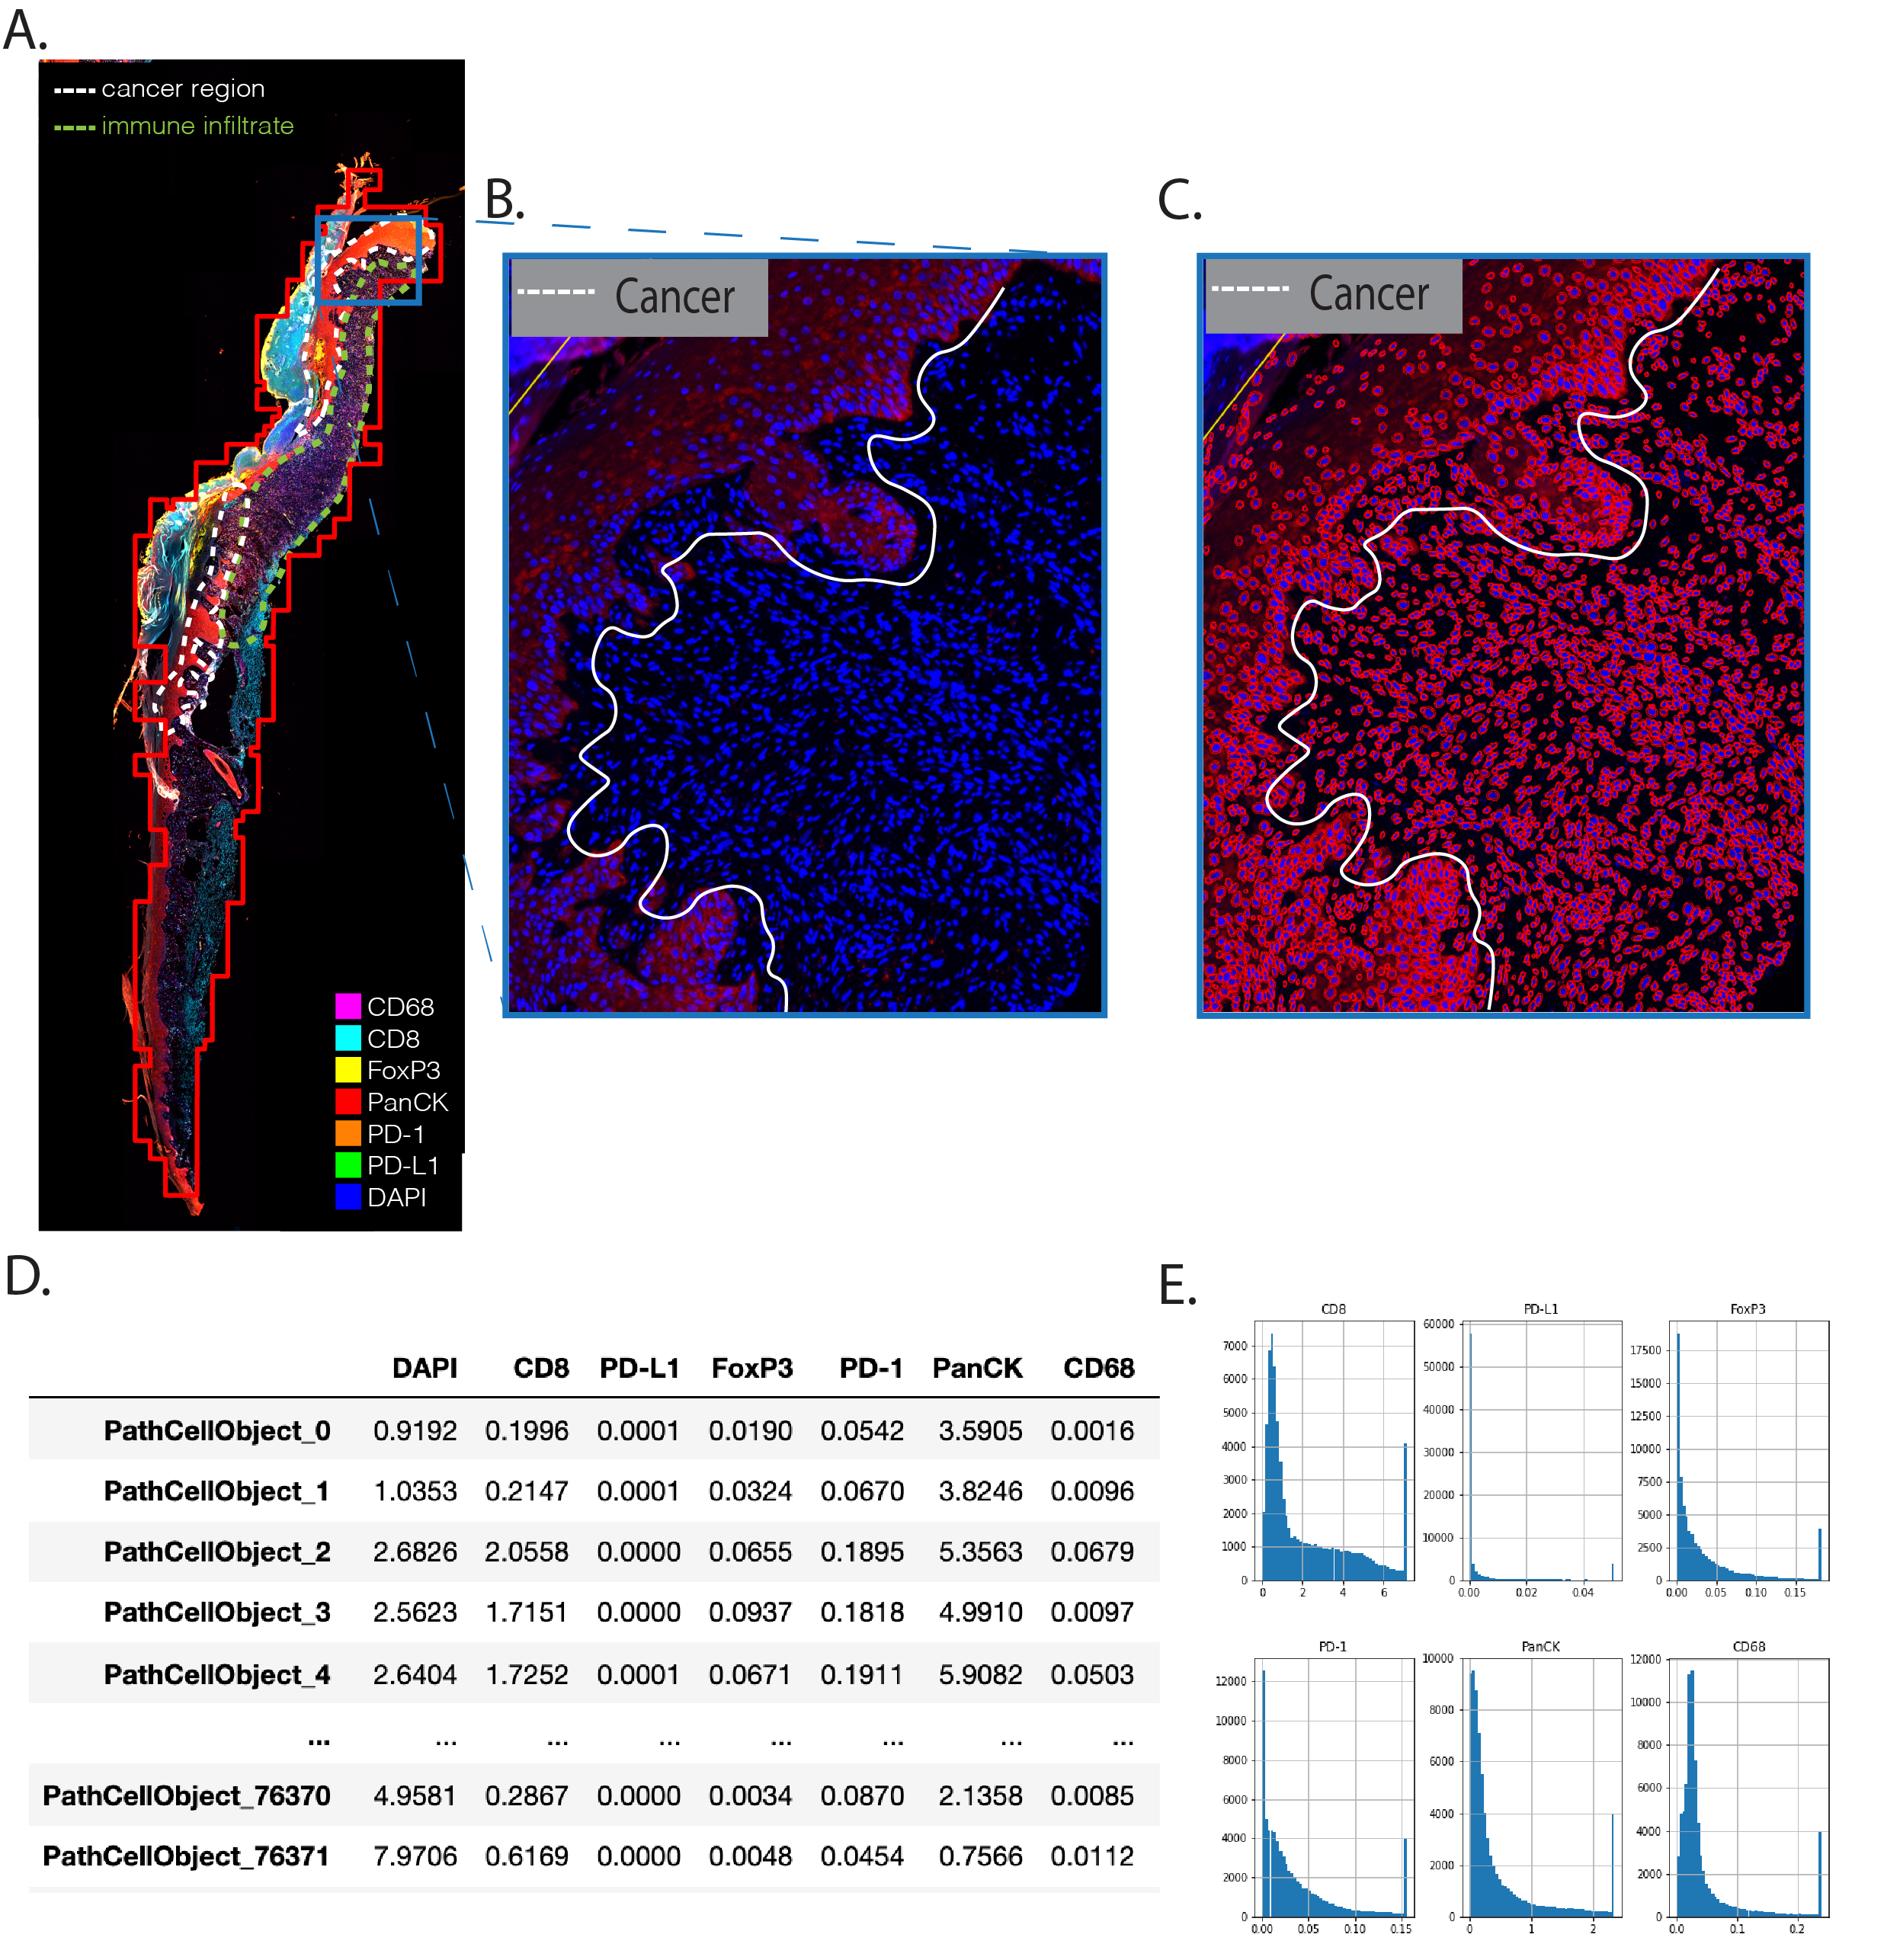
\includegraphics[width=\columnwidth]{Chapter3/Figures/Chap3_Figure1_1.png}
    \caption[Schematic of spatial data preprocessing for cell type annotation.]{ Opal Polaris spatial data preprocessing for cell type annotation. (A) Polaris spatial proteomic data from the SCC patient B18 with the pathological annotation, based on tissue morphology. (B) A zoomed-in image of cell the nuclei representation in DAPI channel (dark blue) and cytokeratin marker expression (PanCK in red) for epithelial cell marker. The annotation line in white colour separates the cancer lesions of the skin from the lower layer. (C) Detection and segmentation of cells from the image using the nuclei channel. (D) The conversion of imaging-based data to single-cell-based data by measuring the level signal each cell expresses within the cell boundary. (E) Histograms of the expression level of each protein in the panels across all the detection cells}
    \label{fig:Polaris_skin_cancer_preprocessing}
\end{figure}

For the first project, each skin cancer sample contained around $40000\sim 79000$ cells per tissue, depending on the size of the whole slide tissue section. To employ the currently established cell clustering and annotation, the multiplexed Polaris image was transformed into non-imaging-based data through the cell segmentation process (Figure: \ref{fig:Polaris_skin_cancer_preprocessing}A-B) \cite{hickey2021strategies}. More specifically, cell segmentation was carried out throughout the tissue using a deep learning model called StarDist \cite{schmidt2018cell}, which eventually turned every nucleus in the DAPI channel into a list of cell objects. For each cell object, the protein signal intensity was normalised to the mean DAPI intensity within the cell boundary and assigned to the expression level of that protein to the cell (Figure: \ref{fig:Polaris_skin_cancer_preprocessing}B-D). To remove the noisy high background from fluorescent intensities (outliers), we added a custom threshold of $95^{th}$ percentile which was used to cap the maximum value of each marker (Figure: \ref{fig:Polaris_skin_cancer_preprocessing}D-E). 

After the raw imaging data were processed and quality checked, single-cell protein expression data were further scaled and clustered using the Leiden clustering algorithm from scanpy \cite{wolf2018scanpy}. The result clusters were assessed to determine cell type identity. Using differential expression analysis of each cluster, we were able to identify six major cell types, including epithelial (PanCK+), inmate immune (CD68+), and adaptive immune (CD8+, FoxP3+) cells from all tissue samples. Cells showing very low expression of all six protein markers were classified as "unidentified" and removed from downstream analysis. The spatial coordinate of each cell was retained to further facilitate the construction of the neighbourhood network and spatial analysis of cell-type colocalisation. 

\subsubsection{Cell segmentation and identification from Imaging Mass Cytometry data}
For our IMC dataset in COAD, the raw data from the imaging system is converted into multichannel images which are later undergone cell segmentation for data preprocessing. One key difference in terms of imaging resolution is that the IMC platform has lower resolution compared to multiplexed Polaris. While every pixel in the Polaris image captures $0.49 \mu m$ in the real tissue, the specification in IMC is $1$pixel representing $1\mu m$. the IMC image generated discrete ion count signals (counts of heavy metal molecules from labelled antibodies) which required a specialised cell segmentation method. Currently, the IMC image conversion and preprocess pipeline are being adapted from a pipeline by Bodenmiller Group, one of the founders of the technology (\href{https://github.com/BodenmillerGroup/ImcSegmentationPipeline/blob/development/scripts/imc_preprocessing.ipynb}{IMC preprocessing pipeline}. 

Briefly, after the raw IMC data (.mcd file) is converted into a standard image format with multiple channels (OME tiffs) and each channel represents the expression of a protein staining marker (Figure \ref{Chap3:fig:IMC_data_preprocessing}A). Because the signal intensity in IMC has a lower resolution yet is noisier than in Polaris, we manually built a segmentation model to assign pixels to either cell nuclei, cytoplasm, or background. In collaboration with a team member, who has a clinical background, we assigned the pixel annotation to a subset of cells in the whole ROI using CellProfiler and Ilastik \cite{carpenter2006cellprofiler, berg2019ilastik}. The trained pixel classification model from Ilastik was performed across the whole dataset to segment the cells from the background (Figure \ref{Chap3:fig:IMC_data_preprocessing}B-D). Since IMC imaging data was generated only for selected ROIs, the number of cells in this project is significantly lower than that in the skin cancer project, ranging from $200$ to $1600$ cells per ROI (approximately 2-3 ROIs per sample). After the cell segmentation, customised single-cell data preprocessing is applied to map signals to a list of cell objects. Cellular data was also clipped to remove outliers. Additionally, cells that were either too small (due to  signal noise) or too large (possibly overlapped cells) were filtered from the downstream analysis (Figure \ref{Chap3:fig:IMC_cell_type_annotation}). By applying the harmony algorithm for single-cell data from multiple rounds of experiments, a total of 903,125 cells were merged for further analysis \cite{korsunsky2019fast}. 

For cell type annotation, major structural cell types were identified with high confidence such as Epithelial/Cancer (E-cadherin and Keratin), Proliferative Tumour (KI67+), and Stromal (Collagen, SM-actin). We were also able to annotate other adaptive like B-cells (CD20), cytotoxic T-cells (CD8+), Lymphocytes (CD4+), Natural Killer cells (FoxP3+), and Macrophages (CD68) (Fig:\ref{fig:colorectal_cancer_IMC}A). For validation, we compared the IMC-identified cell types against pathologist annotation. Through a process called image registration, we were able to align the IMC image to the adjacent section of H\&E image which was annotated with some cell types by the pathologist (Fig:\ref{fig:colorectal_cancer_IMC}B). Since our computational results matched well with manual annotation this gave us confidence in our cell segmentation and clustering approaches before proceeding to the CCC analyses.

\begin{figure}[htp]
    \centering
    \includegraphics[width=0.66\columnwidth]{Chapter3/Figures/imc_histocat_pipeline.png}
    \caption[Illustration of IMC data preprocessing.]{ Summary of the current IMC data preprocessing. (A) Starting from the original IMC from the imaging platform, multi-layer tiff images for the cell segmentation pipeline or single-layer tiff for protein marker visualization. (B) illustrates the cell segmentation process with two steps. The first step involves manual pattern recognition to create the pixel classification mask with Ilastik \cite{berg2019ilastik}. After pixel classification, the pixel probability map is then fed through CellProfiler to generate the mask for each cell in the IMC image. (C) IMC image is highly multiplexing data with each protein signal in an individual tiff image. Therefore we utilise the single-layer tiff image to represent the count/means value of the protein expression in a cell. (D) After the cell segmentation, the protein expression of each cell is measured by projecting each protein channel from the input image to the cell mask.  }
    \label{Chap3:fig:IMC_data_preprocessing}
\end{figure}

\begin{figure}[htp]
    \centering
    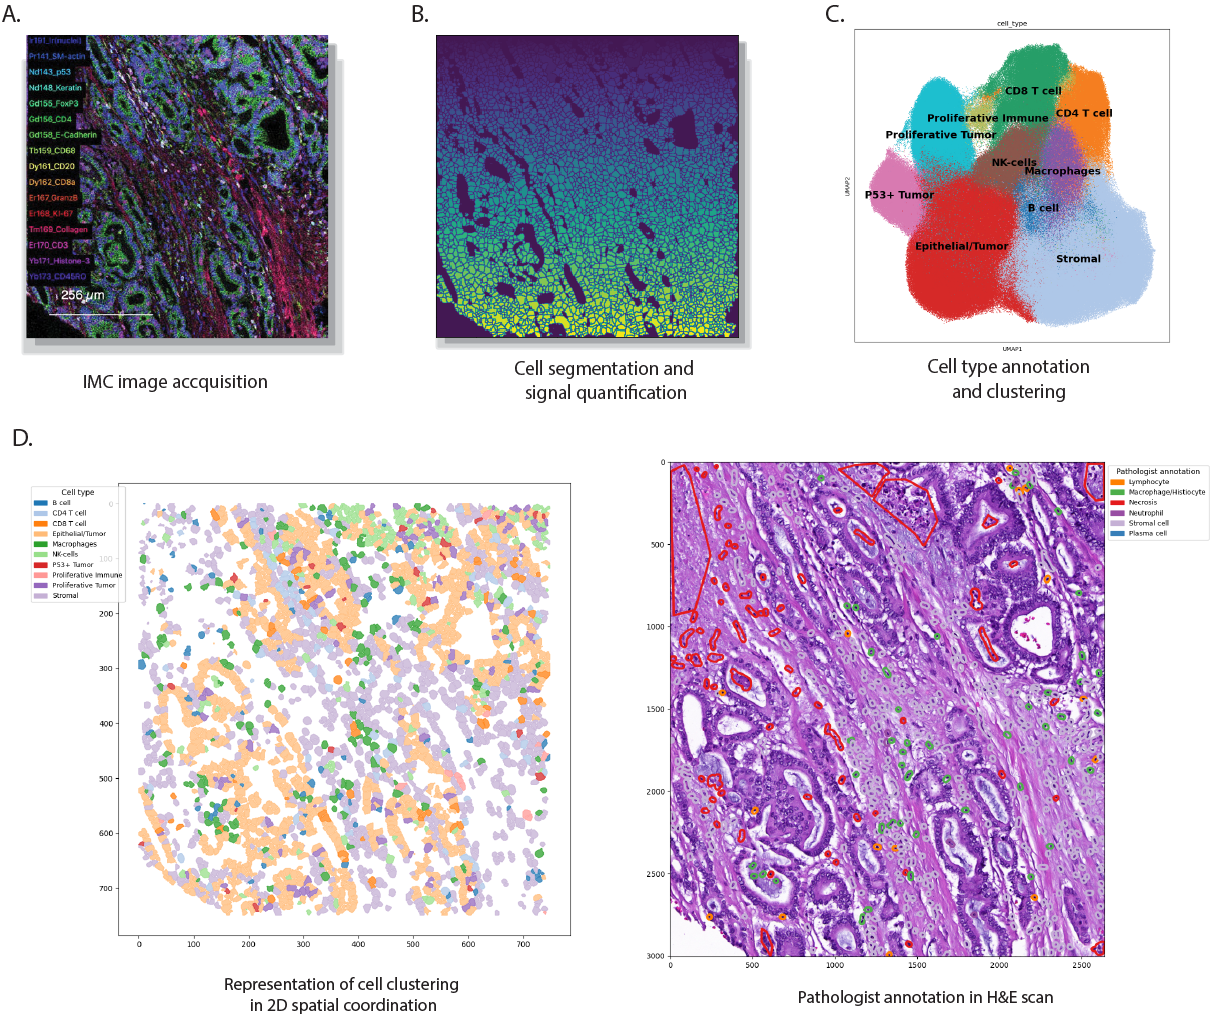
\includegraphics[width=\columnwidth]{Chapter3/Figures/Chapter3_Figure2_IMC_cellID_ver2.png}
    \caption[Hyperion Imaging Mass Cytometry cell identification process]{The workflow for the transformation IMC data from multiplexed imaging data to single-cell proteomic matrix (A) The standard mcd files from Hyperion IMC platform were converted into multiple channel OME-tiff file. Each channel of a tiff image represents a protein staining channel. (B) A pixel classification model was manually generated specifically for the whole dataset to perform cell segmentation. (C) Cells from multiple ROIs were merged, clustered, and annotated. (D) Annotated cells were plotted back to the original spatial context for validation using pathologist annotations.}
    \label{Chap3:fig:IMC_cell_type_annotation}
\end{figure}
\subsection{Spatial cellular network analyses to detect cell communities}
Both cell types and the TMEs are important attributes when evaluating the stage and heterogeneity of cancer at the tissue level. TMEs can segregate the tissue into multiple cell compartments of cancer nest, stromal and normal regions. We reason that different cell types can reside in the same spatial neighbourhood, and the heterotypic interaction of cells within each spatial region can be reflected by the heterogeneity in cancer. To capture the higher-order scale of spatial features of cancer tumours, we performed cell communities detection. More specifically, we leveraged the existing spatial network analysis to construct the cellular neighbourhood network across each tissue sample. Each cell in the tissue is considered a point process in the Cartesian coordinate system and is connected to neighbouring cells in adjacent proximity. After that, we grouped the cells from the same neighbourhood with similar local features into the same community. We reasoned that the cells w Additionally, the projection of cell community will help to elucidate how cells can perform communication and provide the landscape of cell distribution throughout different sites of tissue. 

\subsubsection{Detecting cell clusters and communities in skin cancer using spatial network}
\label{Sec:3_cell_communities_and_coocurrence}	%CREATE YOUR OWN LABEL.
Using the cell type clustering information, we sought to identify the regions where cancer and immune cells were highly co-localised and possibly interacted. First, we investigated cell type co-localisation through spatial clustering analysis \cite{schurch2020coordinated}. The spatial feature of a cell was extracted by scanning $K$ nearest neighbouring cells surrounding the query cells. The nearest neighbour metric was defined by the Euclidean distance between the $X$ and $Y$ coordinates of the cells in the two-dimensional tissue section. For each cell across the tissue, we identified the neighbouring cells using $10$ nearest neighbours within a radius of $100\mu$m from the query cell. The neighbouring profiles of every cell across the tissue were aggregated and clustered using mini-batch $K$ Means clustering. By clustering the cells based on cell neighbourhood profile (e.g. spatial features), we can group the cells with the common colocalisation profiles into the communities of cells. Additionally, we quantitatively measured the cell composition for each spatial community to identify the cell types enriched for each community. 

We employed cell-type co-occurrence analysis to quantitatively measure the changes in cell localisations through different distances radius. The co-occurrence analysis was inspired by an approach introduced by \cite{tosti2021single}, first applied for spatial transcriptomics data of human pancreas \cite{tosti2021single}. Briefly, Ripley's K-function was used to summarise the co-occurrence of specific cell types with all other cell types across increasing distance intervals. The co-occurrence score can be estimated by the Equation \ref{Eq:Cooc_equation}, which is defined by the fraction of the probability of observing a test cell type $exp$ at the presence of a reference cell type $cond$ ($P_{r}(exp|cond)$) over the probability of observing that test cell type $exp$ $P_{r}(exp)$ at the presence of any other cell type within the same distant interval $r$. At a specific distant $r$, $Co_{r}$ indicates how high/low $exp$ and $cond$ cell types co-localised compared to random cell types. The comparison of $Co_{r}$ at an increasing distant radius $r$ shows how the co-localisation of two cell types starts dispersing. By applying the co-occurrence score, we aimed to ascertain whether cell communities identified by the previous analysis followed true spatial patterns. We implemented the function to measure the co-occurrence score using 25$\mu$m interval with $r$ ranging from 0$\mu$m to 300$\mu$m (95\% of the pairwise distance between condition cell type and others). 


\begin{align}
\label{Eq:Cooc_equation}
Co_{r} = \frac{P_{r}(exp|cond)}{P_{r}(exp)} 
% K(t) =  \sum_{i=1}^{n}\sum_{n}^{j}1\{d_{ij} < r\} \\ 
\end{align}

% \subsection{Applying nearest neighbourhood approaches to cell-cell interaction}
% ********* Enter your text below this line: ********
 

\begin{figure}
    \centering
    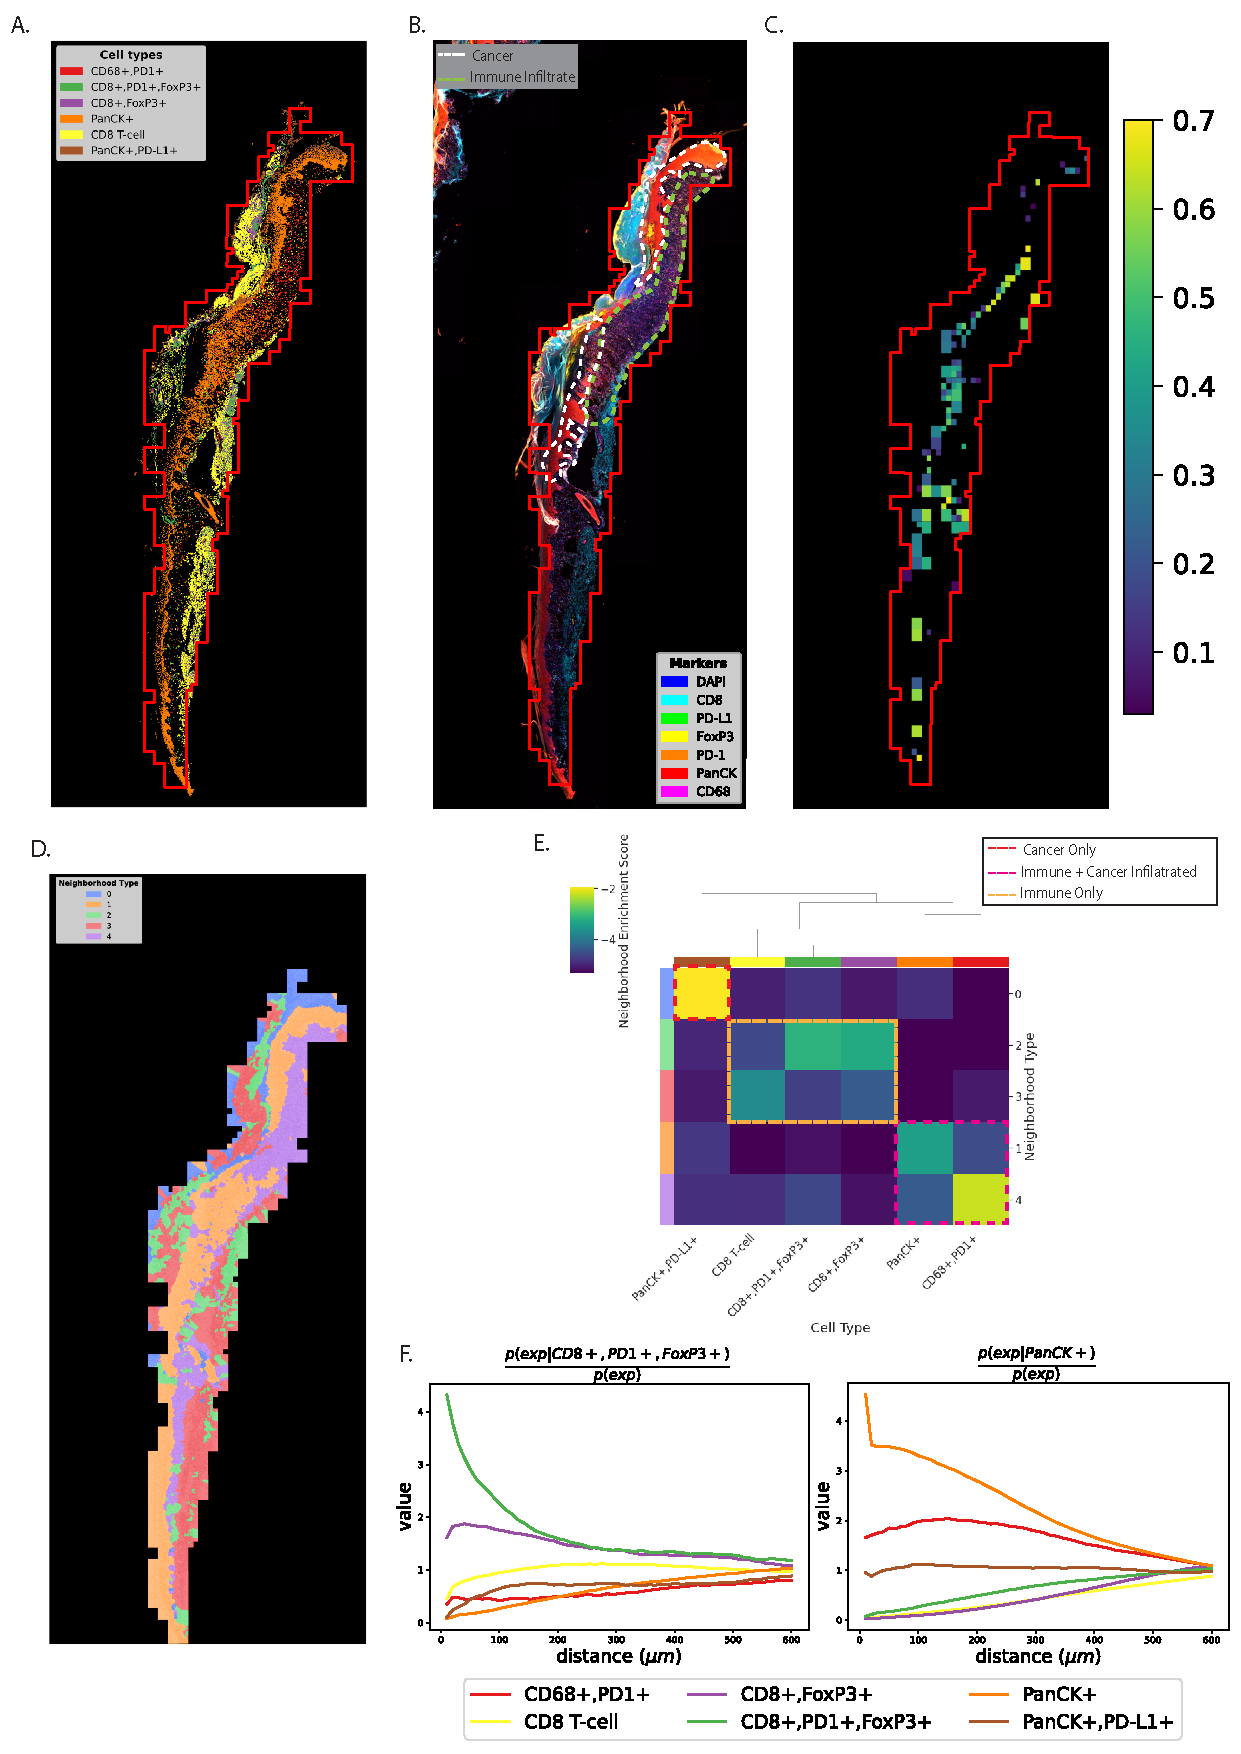
\includegraphics[width=0.8\columnwidth]{Chapter3/Figures/Minh_figure3-01.png}
    \caption[Analyses of Polaris multiplexed imaging of human SCC skin cancer tissue. ]{High-order analyses of Polaris multiplexed imaging data of human SCC skin cancer tissue. (A) Cell type classification through clustering and signal gating of the expression of 6 proteins mapped to single cells. The panel of 6 antibodies was used to profile the protein expression of major interest cell types, including cytokeratin, cancer cells secreting immune inhibitor (PD-L1), and immune cells (CD8 T-cell, NK cells, Macrophages). (B) Pathological annotation of cancer and immune regions, based on tissue morphology. (C) Analysis of cancer-immune cell co-localisation through the ligand-receptor pair PD1 and PD-L1. (D) Voronoi map using the spatial distribution of the cell communities to split the original tissue into multiple regions, representation of distinct cell neighbourhood communities defined via clustering}
    \label{fig:skin_cancer_polaris}
    
\end{figure}

Applying similar cell communities detection and cell type co-occurrence approaches to the COAD project, we sought to test for the co-localization between cancer and immune cells across ROIs. As an example, the general distribution of cells and signals within an ROI is shown in \ref{fig:colorectal_cancer_IMC}A and \ref{fig:colorectal_cancer_IMC}B. Figure \ref{fig:colorectal_cancer_IMC}D shows the probability of observing a cell type conditioned on the presence of cancer cells of the ROIs showed in \ref{fig:colorectal_cancer_IMC}A. We could observe a high enrichment of cancer cells with epithelial cells at the first $200\mu m$ interval. While the co-occurrence analysis could provide insights into how different cell types form cell communities, the analysis is limited to a single ROI at a time. Therefore, we performed an additional analysis where we grouped co-occurrence scores of multiple ROIs together which allowed us to statistically test (Wilcoxon test) for the significance of co-localization relative to the population average. The table embedded in the Figure\ref{fig:colorectal_cancer_IMC}E shows the significant test of occurrence scores between every pair of cell types in our dataset. 

\subsection{Cellular interaction analysis through contact-based approach}
% histocat approach which uses the cell outline
Note that, this approach was applied particularly to the COAD project using the cell mask from cell segmentation as the reference to construct a cell neighbourhood report for each ROI. A we sought to find significantly enriched interactions between or within cell types in the immediate neighbourhood. Firstly, the pairwise interactions of every cell are defined by considering the overlapped cell membrane. Using the extended cell segmentation masks (user-defined threshold), the neighbour interaction is defined as if a pair of cells shared an overlapped in extended cell boundaries. The pairwise interactions are aggregated by the cell types of $observing\_celltype$ and $expecting\_celltype$ and scored by the mean of the total number of $observing\_celltype$. Random permutations were performed by shuffling the cell type of $expecting\_celltype$. For each permutation, the mean of pairwise interaction is calculated again. While the interaction between each pair of cells is bi-direction, the pairwise interaction favours one direction connection originated from $observing\_celltype$. Therefore, the pairwise interaction of random permutation was compared to a baseline distribution using two individual one-tail permutation tests within the same image (each ROI). The $P-values$ suggested how significant a pairwise interaction between a pair of cell types was compared to random, and eventually suggested an interaction or an avoidance. The comparison to a matched randomized tissue for every individual image controls for both the distinct connectivity and the specific cell types in that tissue. By using the extended cell mask boundary, the randomisation process of this neighbourhood analysis approach is not directly affected by absolute cell number or the size of the image. Yet the frequencies of cell types present and the relative quantities are important.

\begin{equation}
\begin{split}
P_{lt} = \frac{ \sum(mean(permutation) \leq mean(real\_data) )}{number\_perm + 1} \\
P_{gt} = \frac{\sum(mean(permutation) \geq mean(real\_data) )}{number\_perm + 1}
\label{chap1:eq:02}
\end{split}
\end{equation}
Where $P_{gt}$ and $P_{lt}$ defined $P$ value for each tail, 
The absolute cell number or the size of the image does not have a direct effect on the neighbourhood analysis; only the frequencies of cell types present and the relative quantities are important. 

\begin{figure}
    \centering
    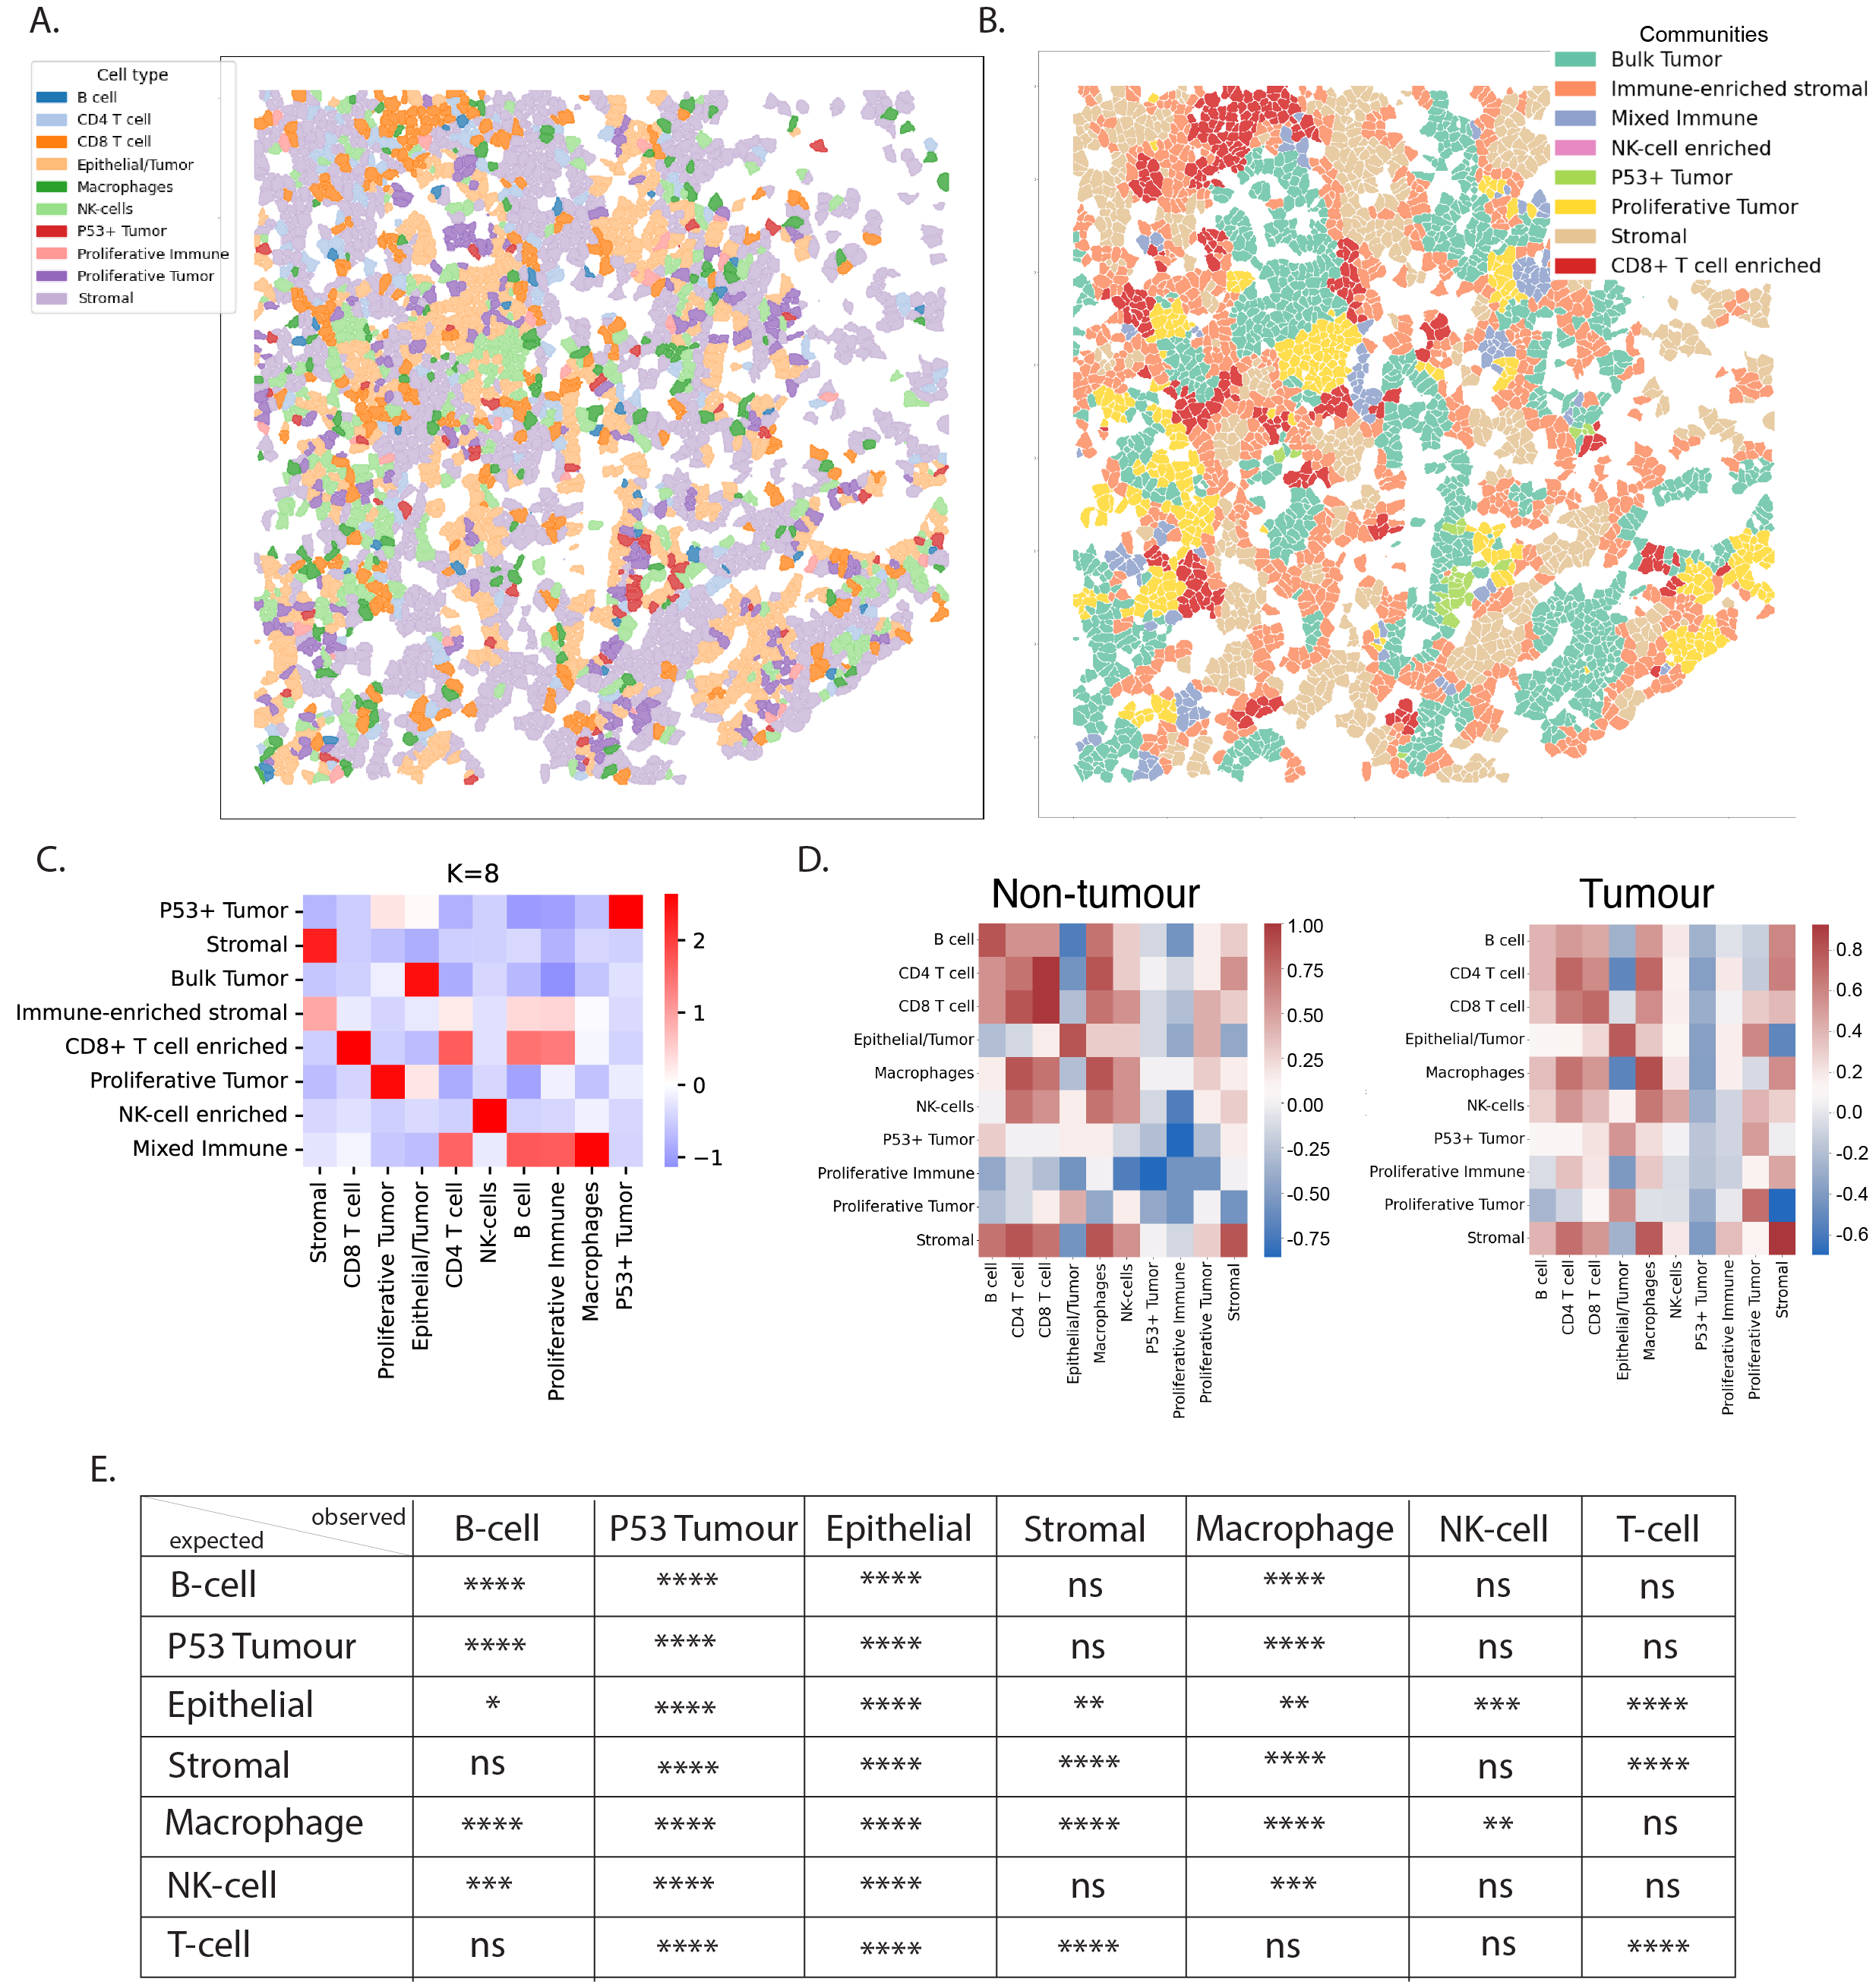
\includegraphics[width=0.8\columnwidth]{Chapter3/Figures/Chap3_figure4_v2.png}
    \caption[High-order cell spatial  analysis result of IMC data.]{High-order cell spatial  analysis result of IMC data (A, B) The cell type and the Voronoi diagram of cell communities detection results of the patient id CR020 (C) The pairwise cell-cell interaction through the contact-based approach. (D) The co-occurrence analysis of different cell types in the presence of cancer cells at increasing distance threshold (E) A summary of significant co-occurrence scores across all combinations of observed and expected cell types.}
    \label{fig:colorectal_cancer_IMC}
    
\end{figure}
% ***************************************************

\subsection{Developing STRISH for cell co-localisation testing using spatial proteomic data}
\label{Sec:3.Cell_colocalisation_PD1_PDL1}	%CREATE YOUR OWN LABEL.
After the first version of the STRISH package, some extended features were made to turn the STRISH pipeline into a more versatile framework. The added functions allowed the STRISH package to handle the spatial proteomic data as the input to perform the analysis. We reasoned that most of the multiplexed imaging technologies which capture gene or protein expression at the subcellular level can be processed through a similar workflow. Collectively, the data preprocessing includes stitching of images, produced by the Polaris, into a multichannel image. Next, cell segmentation and protein expression measurement were applied to turn the imaging data into a single-cell protein expression format \cite{shakya2020immune, liu2019comparison, aghaeepour2013critical}.

After  We applied the scanning window strategy from the STRISH pipeline to the whole slide tissue to identify the co-localisation of PD-L1 positive T-cells (CD8+) and PD1 positive epithelial cells (PanCK+). STRISH starts by dividing the Polaris image into four non-overlapping tiles, each one-fourth of the size of the original slide scan, and gradually splits these large tiles into smaller windows until a predefined cell count threshold is met. The windows containing cells expressed target pairs of proteins, PD1 and PD-L1 are then scored to measure the density of cell type within each window. The scores are then normalised across the windows and used to plot a heatmap showing the co-localisation of the two markers.
\begin{figure}[htp]
    \centering
    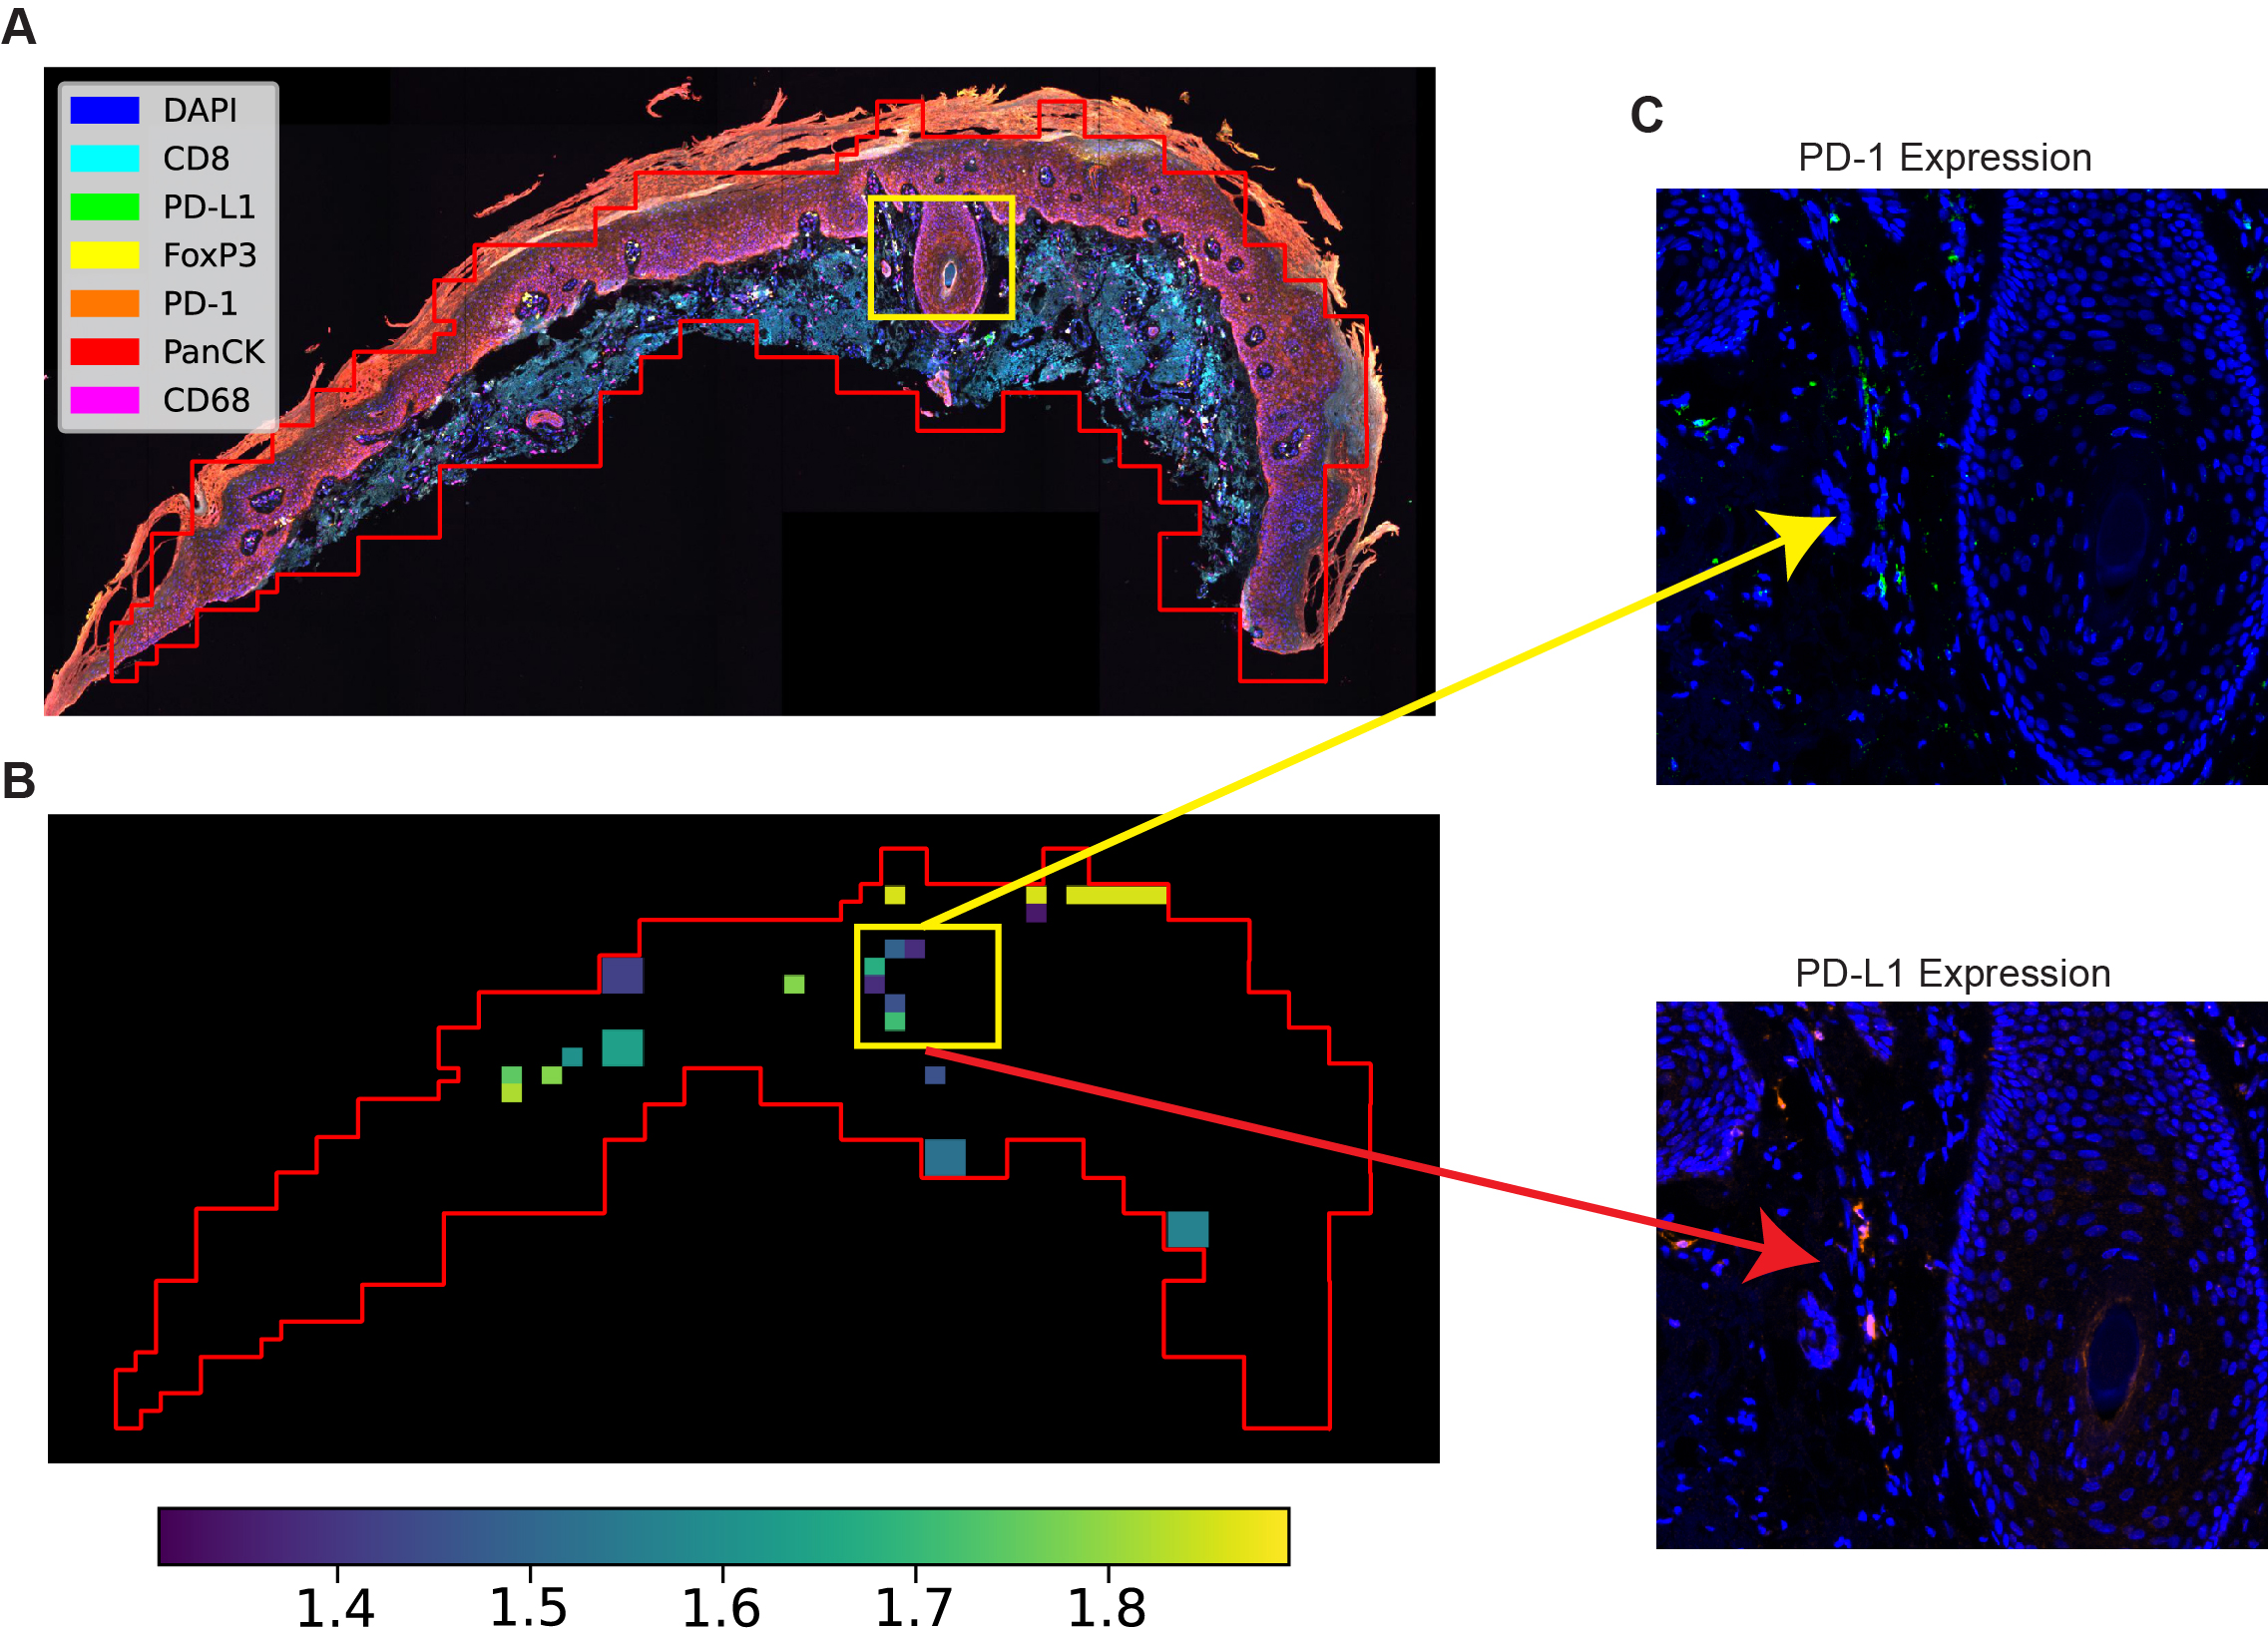
\includegraphics[width=0.8\columnwidth]{Chapter3/Figures/Chapter2_Fig3.jpg}
    \caption[STRISH application to protein data. ]{STRISH application to protein data. (A) A multispectral image captured using MOTiF PD-1/PD-L1 panel (6 proteins and a DAPI) of an SCC cancer tissue section. (B) STRISH significant test heatmap (activity map) suggesting the tissue locations with high (yellow colour) or low (dark colour) level of protein local co-expression after the statistical test for the ligand-receptor pair PD-1 and PD-L1 (the value shows in colour bar indicate negative log p-values). The tissue contour was plotted using the windows of neighbouring cells identified by STRISH. (C) A close-up visualization of the areas identified as the existing cells local co-expression of PD-1 and PD-L1 by STRISH.}
    \label{fig:Chap2_figure3}
\end{figure}

\section{Results}
\subsection{Highly multiplexed Polaris data reveal cell communities in skin cancer}
For the Polaris skin cancer dataset, we identified the cell types that presented using the panel of 6 antibodies. Using Leiden clustering and differential expression analysis of the protein expression between cell clusters, we identified 6 major cell types, including epithelial cells (PanCK+), inmate immune cells (CD68+), and adaptive immune cells (CD8+, FoxP3+) (Fig: \ref{fig:skin_cancer_polaris}A). Among all the clusters detected by the Leiden clustering, those cells with very low expression of all the proteins in the panel were classified as unidentified and removed from downstream analysis. The cell identifications were eventually plotted back to the original spatial context for validation (Fig: \ref{fig:skin_cancer_polaris}B-D).  

Next, we then investigated cell type co-localisation more broadly using spatial community analysis. We performed a clustering analysis to group tissue regions with similar local densities of various cell types, which for patient B18 resulted in the identification of five cell communities distributed across the tissue \ref{fig:skin_cancer_polaris}D). Using the cell communities detection method, we identified five cell communities distributed across the tissue. Quantitative assessment of cell composition in each community allowed us to deduce biologically interpretable features of these communities (Fig: \ref{fig:skin_cancer_polaris}D). Particularly, communities 2 and 3 consisted of scattered immune cells while community 1 appeared to have a very high density of epithelial cells positive with PD-L1. This could be explained by the known biological process and tissue structure that cancerous epithelial cells tend to reside densely around the cancer nest, and the presence of immune cells under the epidermis layer (Fig: \ref{fig:skin_cancer_polaris}B, E). On the other hand, clusters 1 and 4 contain mixed epithelial and immune cell populations in the same communities. Comparing the distribution of cell communities and tissue annotation (Fig: \ref{fig:skin_cancer_polaris}B) suggested that the clusters 2, 3 and 4 highly aligned with the stromal microenvironment communities (Fig: \ref{fig:skin_cancer_polaris}D).  Of note, using our own STRISH test (described in more detail later), we found spatially-specific interactions between PD1 and PDL1 along the edge of cancer and immune cells \ref{fig:skin_cancer_polaris}C).


\subsection{Spatial analysis of Polaris data for profiling cellular interaction via PD1 and PD-L1}
Quantitative assessment of cell composition in each community allowed us to deduce biologically interpretable features of these communities (Fig ). In particular, Community 0 has a very high density of PD-L1+ epithelial cells, while Communities 2 and 3 are enriched for three types of CD8+ T cells. Visual inspection of the location of Communities 2 and 3 reveals their spatial proximity, which may be explained by the tendency of cancerous epithelial cells to reside densely around the cancer nest, and for immune cells to sit under the epidermis layer 36. We also observed that Communities 1 and 4 group together (Fig S12e), and that these communities contain a mixture of both cancer and immune cell populations. The spatial distribution of mixed cancer/immune communities (Fig S12d) aligns with the spatially-specific interaction observed between PD-1 and PD-L1 along the interface between cancer and immune cells (Fig: \ref{fig:skin_cancer_polaris}C).

We further sought to detect the local co-localisation of the L-R pair PD-1 and PD-L1, well-known signalling molecules used in immune and cancer cell interaction \cite{pardoll2012blockade} through applying the STRISH package to spatial proteomic data.  We employed our pipeline, STRISH pipeline, to automatically and unbiasedly detect regions containing T-cells double positive for CD8 and PD-1 in the immediate vicinity of cancerous epithelial cells, which themselves are double positive for PanCK and PD-L1 (Fig \ref{fig:skin_cancer_polaris}C). Interestingly, for patient B18, we found that the PD-1+ immune cells and PD-L1+ epithelial cells mostly co-localised at the interface of cancer and immune infiltration, as defined by a pathologist’s annotation (Fig \ref{fig:skin_cancer_polaris}A). Similar patterns were observed by applying STRISH pipeline to the tissue samples from patients R01 and P04 (Fig: \ref{fig:Chap2_figure3}). 


\subsection{Identifying cell communities through Imaging Mass Cytometry data}
\subsection{Cell co-localisation and neighbourhood enrichment analysis in colorectal cancer }
Using CD8 T-cells positive with PD1+ protein as the condition (reference) cell type), the co-occurrence test confirmed that the co-localisation of these cells with the other two subgroups of T-cells, including double positives CD8+ and FoxP3+ and single positive CD8+ T-cells were higher than random (at distances from $0\mu m$ to $400 \mu m$). Similarly, PanCK+ was also found to be co-occurred with the CD68+ and PD1+ double-positive clusters, consistent with the result from our community detection analysis \ref{fig:Polaris_skin_cancer_preprocessing}.     
% To improve STRISH, Patients diagnosed with advanced BCC/SCC would be beneficial from the successes of immunotherapy observed in melanoma. 
\section{Discussion}
Knowing that the relationship between cancer-immune interaction in cancer and the heterogeneity of cancer is a bi-directional incident. In this chapter, we presented multiple spatial analysis results to identify cell communities and how the cells communicate through distance. As the spatial proteomic platforms perform tissue imaging differently, we addressed some limitations of conversing the imaging data to single-cell data and introduced the data quality control for data preprocessing. Additionally, we demonstrated the power of performing multiple spatial analyses to validate the findings of each other. That allows us to deduce the biological interpretation of the analyses.      

Importantly, the extension of STRISH application to immunofluorescence data suggests the very broad applicability of this analysis pipeline to the vast amount of protein fluorescence imaging data. It is important to acknowledge that package particularly focuses on cell-cell interaction analyses with the application to both spatial transcriptomic and proteomic data. Hence, it should not be used in isolation but in combination with other data normalisation and cell-type clustering tools. Other spatial analysis packages such as Giotto \cite{dries2021giotto} and squidpy \cite{palla2022squidpy} also provide functions for cell neighbourhood enrichment analysis through L-R pair, such functions, however, can be used for the exploratory analysis. Here, we extended the application of the STRISH package which can be incorporated into both data exploration and validation of the cellular interaction through ligand-receptor pair. 

For the second project of IMC for colorectal cancer, a statistical test to combine the multiple ROIs and tissue samples together for survival prediction and clinical outcome is also another analysis that I will implement and present in Chapter \ref{Chap:4}. The next goal of this thesis is to develop a holistic framework to work with multimodal spatial -omic data and discover different characteristics of CCC throughout cancer tissues and across patients. 

% \section{Quantitative and qualitative measurements}
% \label{Sec:3.4_validation}	%CREATE YOUR OWN LABEL.

% \subsection{Quantification of cell communities conserved across patient groups}
% % ********* Enter your text below this line: ********
% We introduce 
% \subsection{Comparison of tissue heterogeneity across patients and cancer subtypes}
% % ********* Enter your text below this line: ********
% By aggregating cell's neighbourhood from multiple ROIs, STRISH allows the spatial differential analysis across the  conditions and uncover the relationship between treatment outcome and spatial organisation of cell types.

% \section{Appendix}
\begin{figure}[htp]
\renewcommand{\figurename}{Figure}
    \centering
    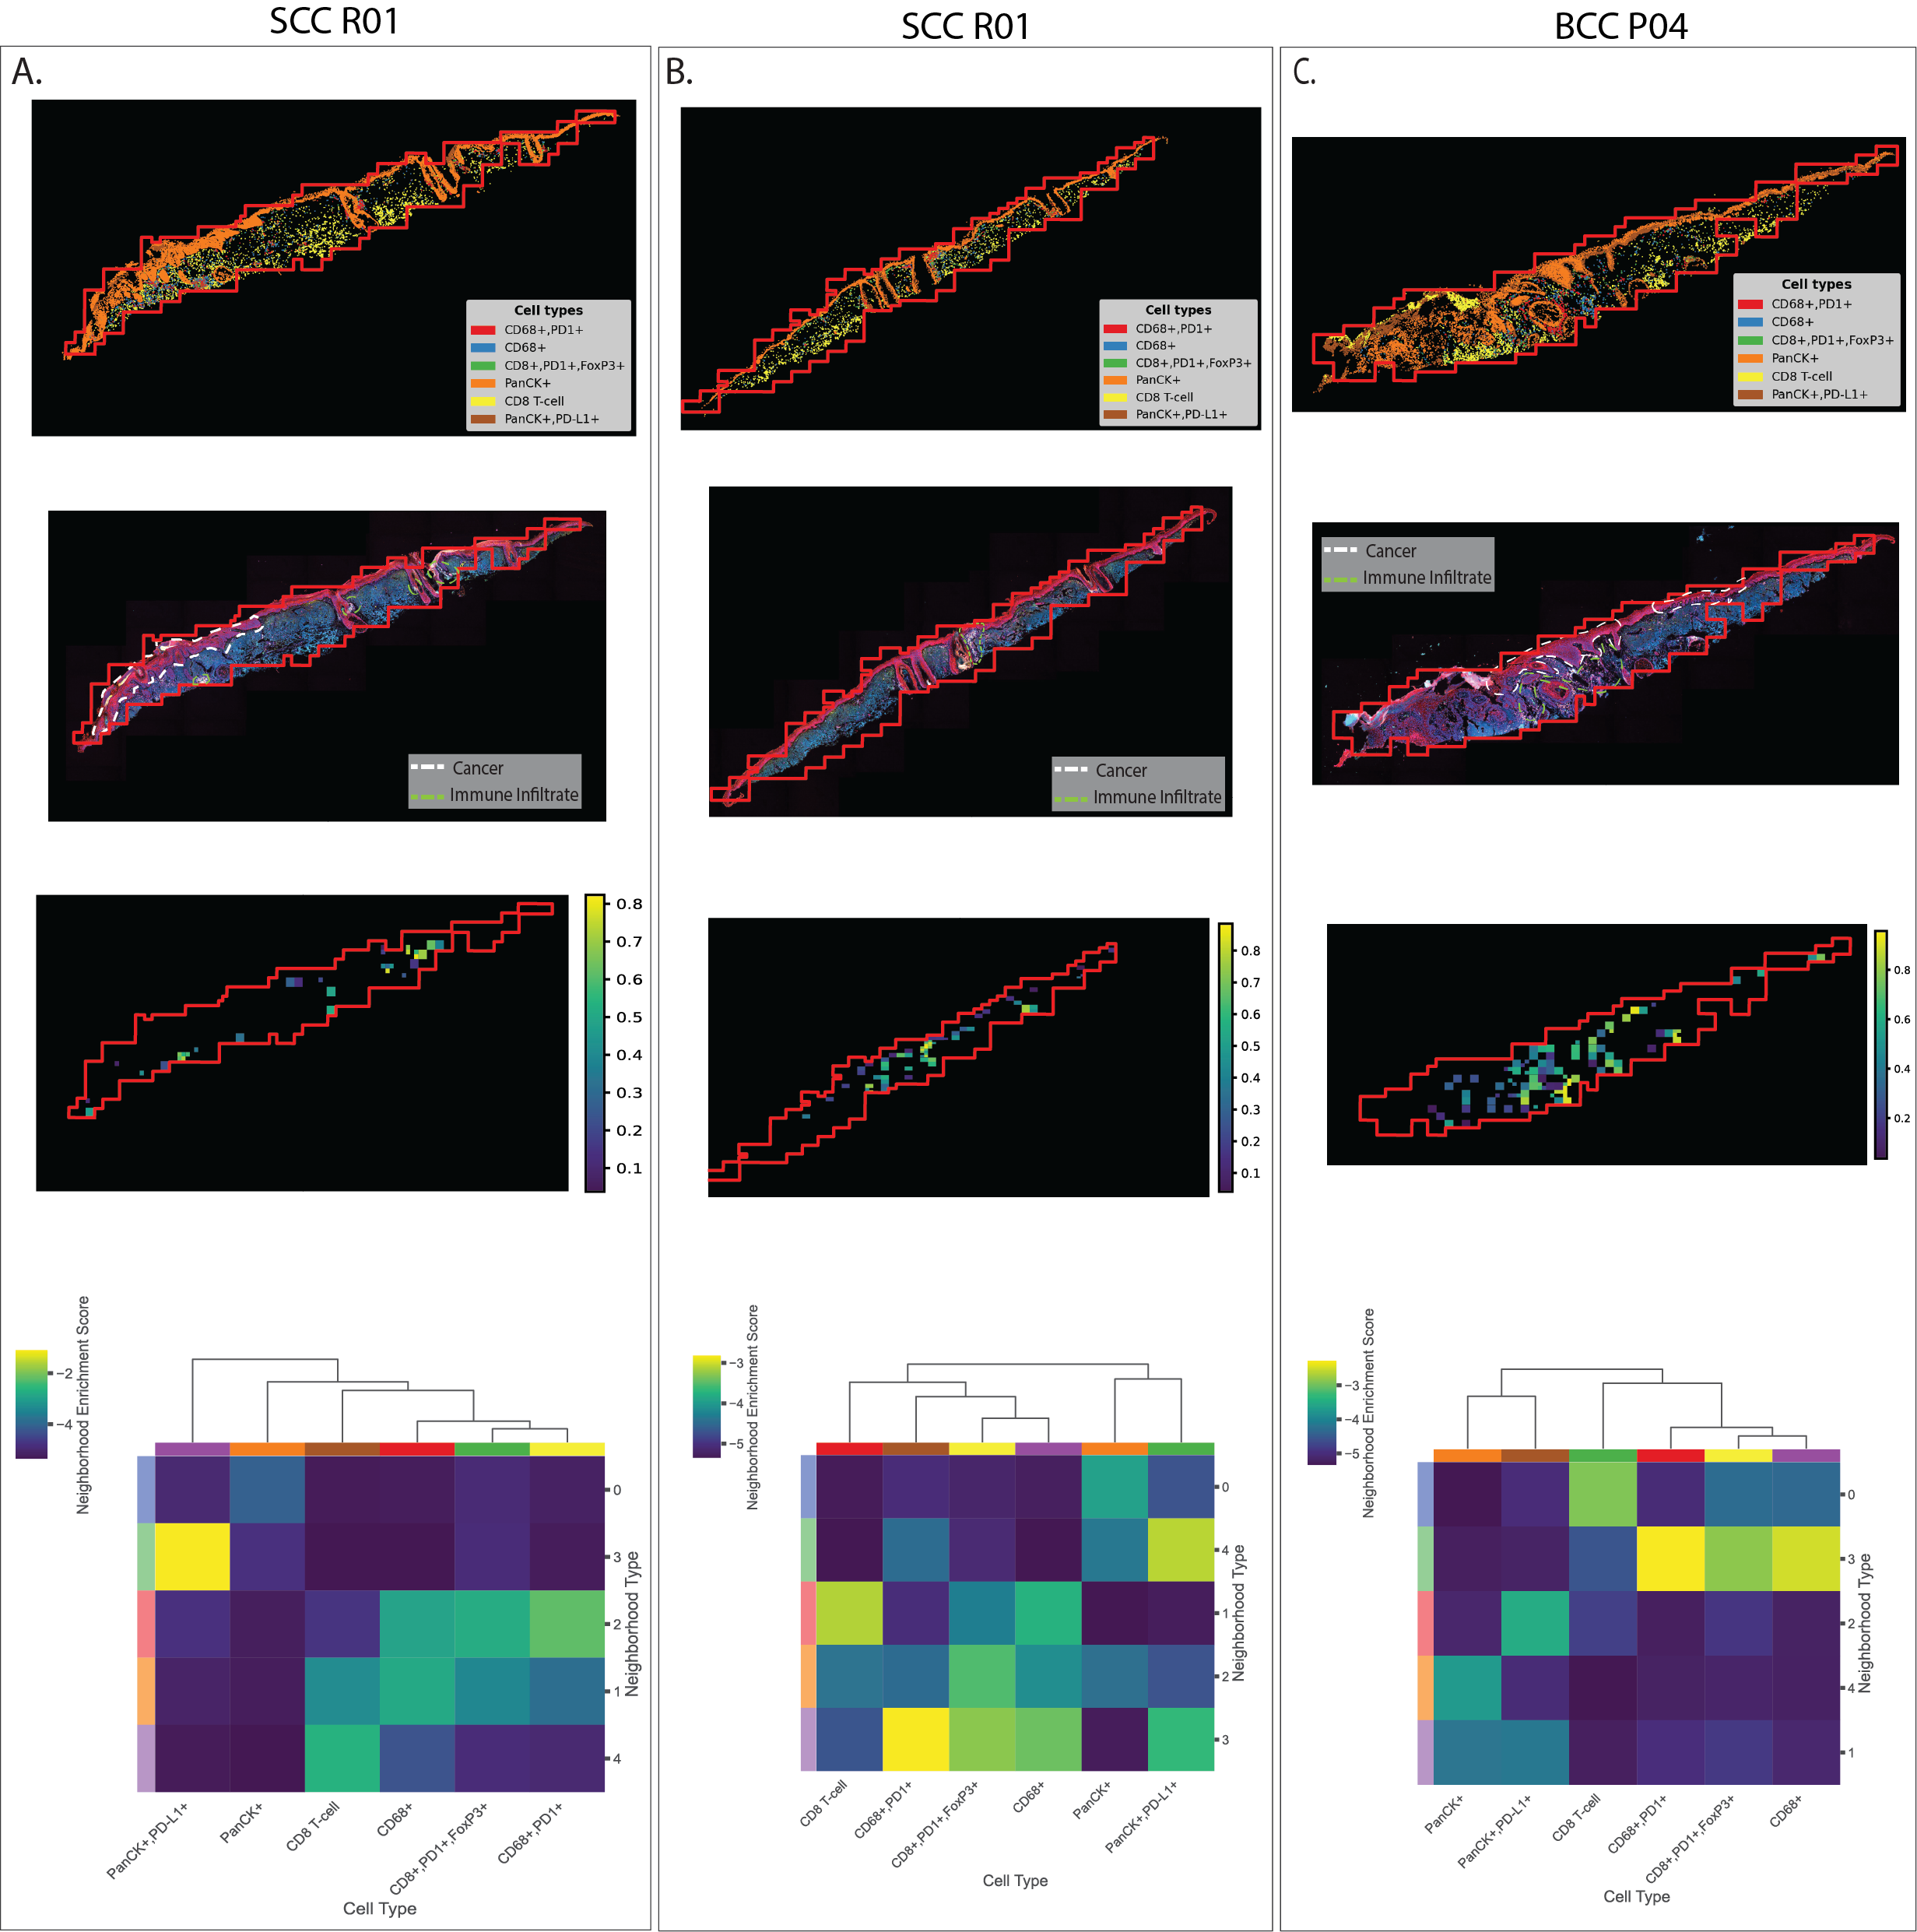
\includegraphics[width=0.75\columnwidth]{Chapter3/Figures/Chap3_supple_figure_1.png}
    \caption[Analyses results of Polaris across multiple SCC and BCC samples]{Analyses results of Polaris across multiple SCC and BCC samples. (A,B) From top to bottom are the cell type identification, pathologist annotation, the heatmap of cell colocalisation through the pair of PD1-PDL1, and the cell type composition for each cell type community detected across the tissue sample from the patient ID R01 with SCC. (C) The equivalent analysis results for the tissue samples from the patient ID P04 with BCC}
    \label{fig:Chap3_figure6}
\end{figure}
% ***************************************************
\section{Appendix}
\begin{figure}[htp]
\renewcommand{\figurename}{Figure}
    \centering
    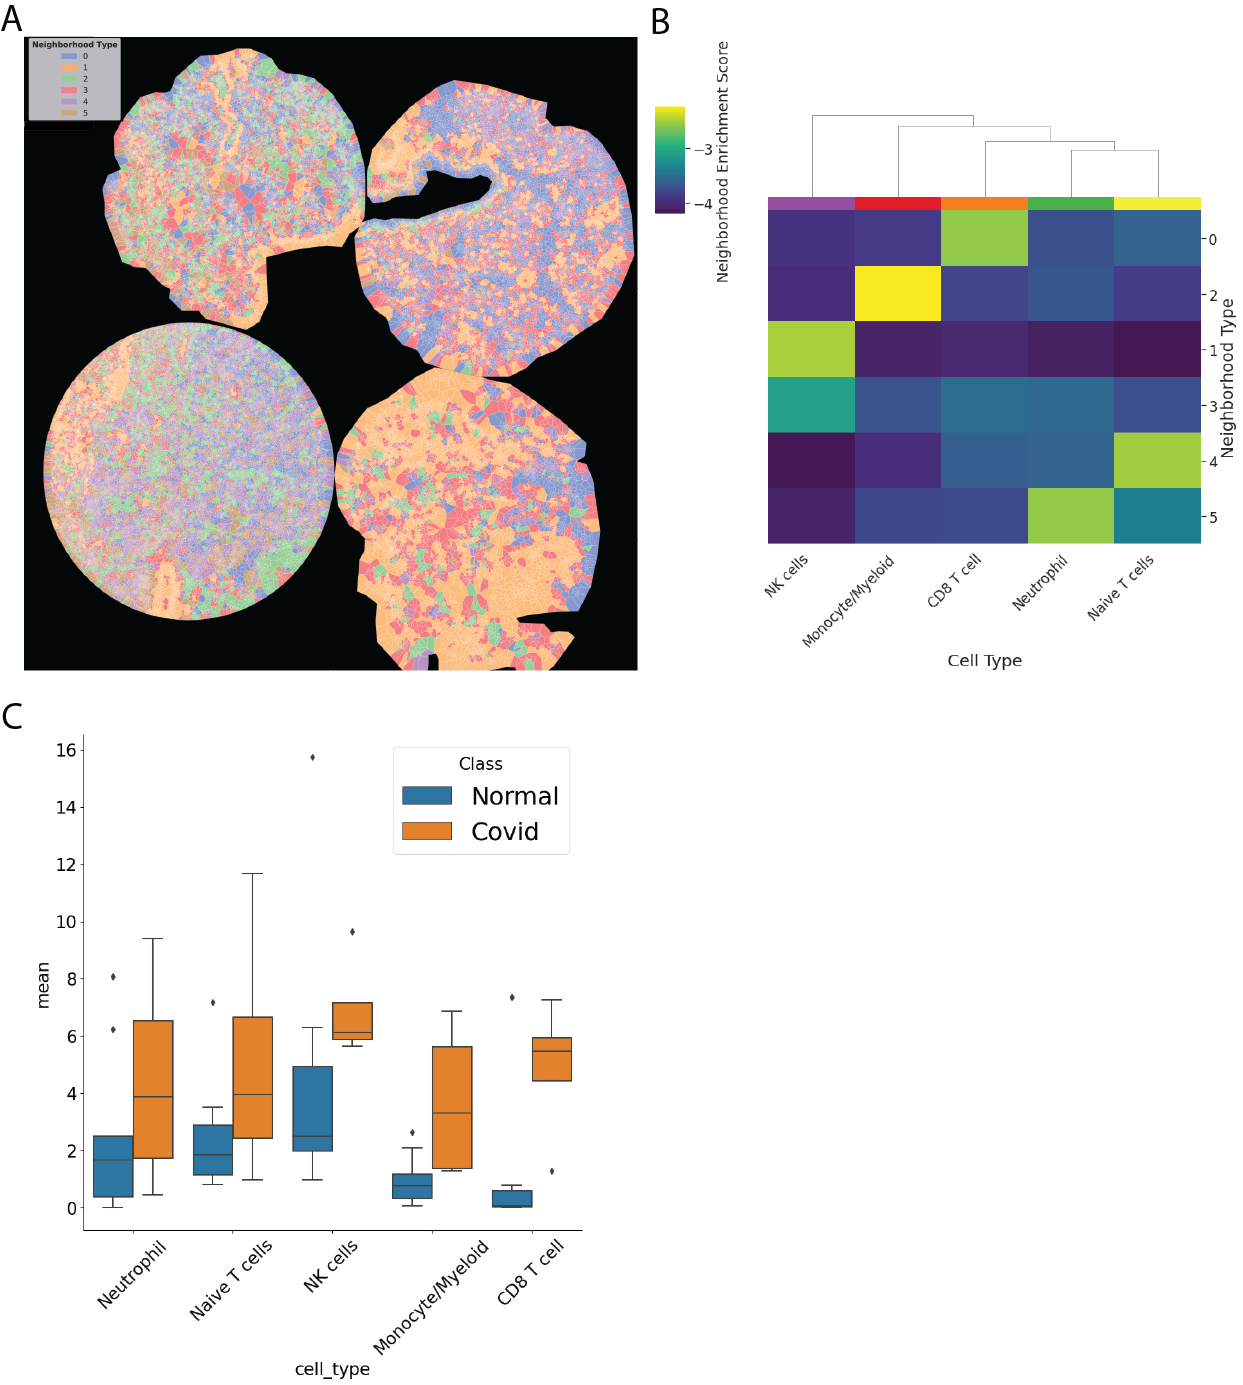
\includegraphics[width=0.75\columnwidth]{Chapter3/Figures/Chap3_Apendix_covid.png}
    \caption[Analyses results in Covid tissue samples using multiplexed Polaris]{Analyses results in Covid lung tissue samples using multiplexed Polaris. (A) Voronoi diagram of cell communities detection in Covid samples. (B) Comparison of cell type detected between Covid infected and normal samples. (C) Heatmap of cell type decomposition of each cell community detected in (A).}
    \label{fig:Chap3_Covid_project}
\end{figure}

% \bibliographystyle{elsarticle-num}

% \bibliography{./References/Bibliography}

% There are already a few computational methods that used scRNA-seq to infer the CCC i.e. CellChat \cite{jin2021CellChat}, CellPhoneDB \cite{efremova2020cellphonedb} or NicheNet \cite{browaeys2020nichenet}. However, they are all unable to address the spatial constraints of interactions. With scRNA-seq data, the limited insights into the spatial location of the RNA molecules within a cell and the organization of cells in a tissue prevent the CCC inference from reaching its potential. To address this, the development of higher multiplexed histological techniques for capturing transcriptomic or/and proteomic information at subcellular resolution, e.g. co-detection by imaging (CODEX) \cite{goltsev2018CODEX} or IMC from Hyperion, facilitated the integration of spatial information into CCC inference. 

% Despite the rapidly growing number of spatially resolved transcriptomic and proteomic technologies, the currently available analysis strategies to process these high dimensional data have not yet exploited the full potential of spatial information. In short, spatially resolved CCC analysis can be categorised into two main categories. The first approach considers each cell as a point in Cartesian coordinate system and assesses the changes in the spatial co-localisation between pairs of cell types at distances \cite{arnol2019modeling,schurch2020coordinated}. Meanwhile, the second category considers the interactions of individual cells and their intermediate adjacent cells within a short proximity from the cell membrane. It is sufficient to measure cell-cell interaction through gap junction or paracrine signalling. The pairwise interaction of two cell types is then grouped by cell phenotypes and compared to randomised labels of cells to determine the significance of interactions  \cite{schapiro2017histocat}. In the following sections, I will go deeper into the advantages and disadvantages of each approach and how I applied them throughout my second-year projects.    

% PD1 has been extensively studied and identified as immune inhibitor for skin cancer cell growth\cite{ishida1992induced,  tsai2014pd}. In the first project using skin cancer as the model to study, we were interested in finding and validating the immune-cancer cell interactions pairing the ligand-receptor PD-L1 and PD1 through a series of spatial analysis methods. On the other hand, we sought to find the pattern of intercellular architecture in colorectal cancer and the correlation between alterations in CCC and the prognosis for the patients. Once the cells were clustered and annotated appropriately, we to applied multiple spatial analyses to study cell-cell interactions with the aim of improving the capability to predict the clinical outcome. For each project, we performed two to three neighbourhood analyses to explore and quantify the tissue section finds.  